\documentclass{article}
\usepackage[utf8]{inputenc}
\usepackage{enumitem}
\usepackage{amsmath}
\usepackage{amsthm}
\usepackage{amssymb}
\usepackage{tikz}
\usepackage{standalone}
\newtheorem{theorem}{Theorem}[section]
\newtheorem{lemma}[theorem]{Lemma}
\setlength{\parskip}{1em}

%------------tikz Setup------------

\tikzstyle{ball} = [circle,shading=ball, ball color=black,
    minimum size=1mm,inner sep=1.3pt]
\tikzstyle{miniball} = [circle,shading=ball, ball color=black,
    minimum size=1mm,inner sep=0.5pt]
\tikzstyle{mminiball} = [circle,shading=ball, ball color=black,
    minimum size=0.6mm,inner sep=0.1pt]
\usetikzlibrary{arrows.meta}
\usetikzlibrary{angles, quotes}
\tikzset{>={Latex[length=2mm,width=1.5mm]}}
\tikzset{->-/.style={decoration={markings, mark=at position #1 with
  {\arrow{>}}},postaction={decorate}}}
\usetikzlibrary{decorations.pathmorphing}
\usetikzlibrary{decorations.pathreplacing}
\usetikzlibrary{arrows.meta,calc}
\usetikzlibrary{bending}
\usetikzlibrary{decorations.markings,shapes.geometric}
\tikzset{->-/.style={decoration={markings, mark=at position #1 with
  {\arrow{>}}},postaction={decorate}}}
\tikzset{-|-/.style={decoration={markings, mark=at position #1 with
  {\arrow{stealth}}},postaction={decorate}}}
\tikzset{movearrow/.style 2 args ={
        decoration={markings,
    mark= at position {#1} with {\arrow{#2}} ,
        },
        postaction={decorate}
    }
}

\renewcommand\qedsymbol{$\blacksquare$}

\title{REU 2021 - Problem Set 4}
\author{Kevin Y. Wu}
\date{\today}

\begin{document}

\maketitle

\pagenumbering{roman}
\tableofcontents
\newpage
\pagenumbering{arabic}


\section{Problem 1.}
Consider two lines in the plane with the angle $\gamma$ between them and suppose a grasshopper is jumping from one line to the other. Every jump is exactly $30$ inches long, and the grasshopper jumps backwards whenever it has no other options. Prove that the sequence of its jumps is periodic if and only if $\frac{\gamma}{\pi}$ is a rational number.
\begin{proof}
We can consider each jump as a vector of length $30$ inches. Call the two lines $\ell_1$ and $\ell_2$, and the angle between them $\gamma$. Consider all jumps as vectors. Suppose the grasshopper starts at point $a_1$ on $\ell_1$ and jumps along vector $\overrightarrow{v}_1$ to point $a_2$ on $\ell_2$. Then let $\overrightarrow{v}_2$ be the reflection of $\overrightarrow{v}_1$ over $\ell_1$. 
\par Let $\ell_2'$ be the reflection of $\ell_2$ over $\ell_1$ and draw two vectors $\overrightarrow{v}_1'$ and $\overrightarrow{v}_2'$ of length $30$ that meet at point $a_3$ on $\ell_1$. We see that the shape formed is a rhombus, so $\overrightarrow{v}_2'=\overrightarrow{v}_2$. Hence, by the reflecting a vector about the line on which its head lies, we obtain the vector of the next jump.

\begin{figure}[h]
    \centering
    \documentclass{standalone}
\usepackage{tikz}
\usepackage{graphicx}  
%------------tikz Setup------------

\tikzstyle{ball} = [circle,shading=ball, ball color=black,
    minimum size=1mm,inner sep=1.3pt]
\tikzstyle{miniball} = [circle,shading=ball, ball color=black,
    minimum size=1mm,inner sep=0.5pt]
\tikzstyle{mminiball} = [circle,shading=ball, ball color=black,
    minimum size=0.6mm,inner sep=0.1pt]
\usetikzlibrary{arrows.meta}
\usetikzlibrary{angles, quotes}
\tikzset{>={Latex[length=2mm,width=1.5mm]}}
\tikzset{->-/.style={decoration={markings, mark=at position #1 with
  {\arrow{>}}},postaction={decorate}}}
\usetikzlibrary{decorations.pathmorphing}
\usetikzlibrary{decorations.pathreplacing}
\usetikzlibrary{arrows.meta,calc}
\usetikzlibrary{bending}
\usetikzlibrary{decorations.markings,shapes.geometric}
\tikzset{->-/.style={decoration={markings, mark=at position #1 with
  {\arrow{>}}},postaction={decorate}}}
\tikzset{-|-/.style={decoration={markings, mark=at position #1 with
  {\arrow{stealth}}},postaction={decorate}}}
\tikzset{movearrow/.style 2 args ={
        decoration={markings,
    mark= at position {#1} with {\arrow{#2}} ,
        },
        postaction={decorate}
    }
}


\begin{document}
\begin{tikzpicture}
\begin{scope}[scale=4]
    %lines
    \draw [<->] (-1.8, 0) -- (0.5, 0);
    \draw [<->] (-1.5, -0.75) -- (0.5, 0.25);
    \draw [<->, dashed] (-1.5, 0.75) -- (0.5, -0.25);
    \node[right] at (0.5, 0) {$\ell_1$};
    \node[right] at (0.5, 0.25) {$\ell_2$};
    \node[right] at (0.5, -0.25) {$\ell_2'$};
    \node (o) at (0, -0) {};
    %vectors
    \node[ball,label={above right:$a_1$}] (a1) at (-0.5, 0) {};
    \node[ball,label={below right:$a_2$}] (a2) at (-0.8, -0.4) {};
    \node[ball,label={above:$a_2'$}] (a2') at (-0.8, 0.4) {};
    \node[ball,label={above left:$a_3$}] (a3) at (-1.1, 0) {};
    \node[ball,label={above left:$a_4$}] (a4) at (-1, -0.5) {};
    \node[ball,label={below right:$a_3'$}] (a3') at (-0.66, -0.88) {};
    \draw[->, dashed] (a1) to (a2');
    \draw[->, dashed] (a2') to (a3);
    \draw[->] (a1) to (a2);
    \draw[->] (a2) to (a3);
    \draw[->, dashed] (a2) -- (a3');
    \draw[->, dashed] (a2) -- (a3');
    \draw[->] (a3) to (a4);
    \draw[->, dashed] (a3') to (a4);
    % angle
    \pic [draw,
          angle radius=4mm, angle eccentricity=1.2,
          "${\scriptstyle \theta}$"] {angle = a3--a1--a2};
    \pic [draw,
          angle radius=4mm, angle eccentricity=1.2,
          "${\scriptstyle \theta}$"] {angle = a2'--a1--a3};
    \pic [draw,
          angle radius=4mm, angle eccentricity=1.2,] {angle = a3--a2--a4};
    \pic [draw,
          angle radius=5mm, angle eccentricity=1.2,
          "${\scriptstyle \gamma}$"] {angle = a1--o--a2};
    \node (x) at (-0.95, -0.35) {${\scriptscriptstyle \theta+\gamma}$};
    %vector labels
    \node (v1) at (-0.54, -0.18) {$\overrightarrow{v}_1$};
    \node (v2) at (-0.87, -0.2) {$\overrightarrow{v}_2$};
    \node (v3) at (-1.12, -0.23) {$\overrightarrow{v}_3$};
\end{scope}
\end{tikzpicture}
\end{document}
    \caption{First three jumps of a grasshopper.}
\end{figure}

\par Equivalently, this is a rotation $R_1$ about angle $2\theta$. Without loss of generality, let this rotation be clockwise, as in the diagram below. By drawing a line parallel to $\ell_2$ from $a_2$, we can see that the angle formed between $\overrightarrow{v}_2$ and $\ell_2$ is $\theta+\gamma$. Thus, $\overrightarrow{v}_3$ is a counterclockwise rotation $R_2$ of $\overrightarrow{v}_2$ about angle $2\theta+2\gamma$. Similarly, $\overrightarrow{v}_4$ is a clockwise rotation $R_3$ of $\overrightarrow{v}_3$ about angle $2\theta+4\gamma$, $\overrightarrow{v}_5$ is a counterclockwise rotation $R_4$ of $\overrightarrow{v}_4$ about angle $2\theta+6\gamma$, and so forth. Then
\begin{align*}
    (R_2\circ R_1)(\overrightarrow{v}_1) &= R_{2\gamma}(\overrightarrow{v}_1)=\overrightarrow{v_3}.\\
    (R_4\circ R_3)(\overrightarrow{v}_3) &= R_{2\gamma}(\overrightarrow{v}_3)=\overrightarrow{v_5}=R_{4\gamma}(\overrightarrow{v}_1).\\
    \dots
\end{align*}
\par For the sequence of jumps to be periodic, the grasshopper must eventually return to point $a_1$, so there are an even number of jumps in the sequence, say $2n$. If we group every two consequent rotations starting from $R_2\circ R_1$ as above, to return to the beginning of the sequence, we must have 
\[\overrightarrow{v}_1=R_{2n\gamma}(\overrightarrow{v}_1).\]
\par Hence, $2n\gamma=0\mod{2\pi}$, so $\frac{\gamma}{\pi}$ is a rational number.
\end{proof}


\section{Problem 2.}
Let $ABCD$ be a convex $4-$gon and consider four squares constructed on the outside of each of its edges. Prove that the segments connecting the centers of the opposite squares are mutually perpendicular and equal in length.

\begin{figure}[h]
    \centering
    \documentclass{standalone}
\usepackage{tikz}
%------------tikz Setup------------

\tikzstyle{ball} = [circle,shading=ball, ball color=black,
    minimum size=1mm,inner sep=1.3pt]
\tikzstyle{miniball} = [circle,shading=ball, ball color=black,
    minimum size=1mm,inner sep=0.5pt]
\tikzstyle{mminiball} = [circle,shading=ball, ball color=black,
    minimum size=0.6mm,inner sep=0.1pt]
\usetikzlibrary{arrows.meta}
\usetikzlibrary{angles, quotes}
\tikzset{>={Latex[length=2mm,width=1.5mm]}}
\tikzset{->-/.style={decoration={markings, mark=at position #1 with
  {\arrow{>}}},postaction={decorate}}}
\usetikzlibrary{decorations.pathmorphing}
\usetikzlibrary{decorations.pathreplacing}
\usetikzlibrary{arrows.meta,calc}
\usetikzlibrary{bending}
\usetikzlibrary{decorations.markings,shapes.geometric}
\tikzset{->-/.style={decoration={markings, mark=at position #1 with
  {\arrow{>}}},postaction={decorate}}}
\tikzset{-|-/.style={decoration={markings, mark=at position #1 with
  {\arrow{stealth}}},postaction={decorate}}}
\tikzset{movearrow/.style 2 args ={
        decoration={markings,
    mark= at position {#1} with {\arrow{#2}} ,
        },
        postaction={decorate}
    }
}


\begin{document}
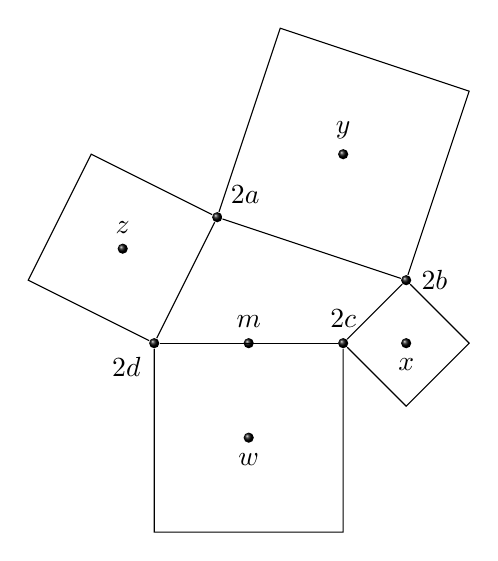
\begin{tikzpicture}
\begin{scope}[scale=0.4]
    %vertices
    \node[ball, label={above right:$2a$}] (A) at (-1,3) {};
    \node[ball, label={right:$2b$}] (B) at (5,1) {};
    \node[ball, label={$2c$}] (C) at (3,-1) {};
    \node[ball, label={below left:$2d$}] (D) at (-3,-1) {};
    %midpoint
    \node[ball, label={above:$m$}] (m) at (0,-1) {};
    %centers
    \node[ball, label={below:$w$}] (w) at (0,-4) {};
    \node[ball, label={below:$x$}] (x) at (5,-1) {};
    \node[ball, label={above:$y$}] (y) at (3,5) {};
    \node[ball, label={above:$z$}] (z) at (-4,2) {};
    %squares
    \draw (A) -- (1,9) -- (7,7) -- (B);
    \draw (D) -- (-7,1) -- (-5,5) -- (A);
    \draw (B) -- (7,-1) -- (5,-3) -- (C);
    \draw (C) -- (3,-7) -- (-3,-7) -- (D);
    %quadrilateral 
    \draw (A) to (B);
    \draw (B) to (C);
    \draw (C) to (D);
    \draw (D) to (A);
\end{scope}
\end{tikzpicture}
\end{document}
    \caption{Polygon $ABCD$ and four constructed squares}
\end{figure}

\begin{proof}
Draw $ABCD$ on the complex plane, and denote its vertices as complex numbers $2a, 2b, 2c, 2d$. Denote the centers of the squares constructed on the outside of its edges $w,x,y,z$. The midpoint of $\overline{AB}$ is $m=\frac{2a+2b}{2}=a+b$. Then the vector from $2a$ to $m$ is $a+b-2a=b-a$, and the vector $\overline{mw}=-i(b-a)=(a-b)i$, since rotation by $90^{\circ}$ in the complex plane is equivalent to multiplication by $-i$. Then by vector addition, we have $w=a+b+(a-b)i$. Doing this for each square's center, we have
\begin{align*}
    w &=a+b+(a-b)i.\\
    x &=b+c+(b-c)i.\\
    y &=c+d+(c-d)i.\\
    z &=d+a+(d-a)i.
\end{align*}
\par Then the segments connecting the centers of opposite squares are represented by the vectors
\begin{align*}
    y-w&=c+d-a-b+(c-d-a+b)i.\\
    z-x&=d+a-b-c+(d-a-b+c)i.
\end{align*}
\par Hence, $z-x=-i(y-w)$, so the vector $\overline{zx}$ is the vector $\overline{yw}$ rotated $90^{\circ}$ clockwise. Thus, the segments connecting the centers of opposite squares are mutually perpendicular and equal in length.
\end{proof}


\section{Problem 3.}
Prove that a composition of three symmetries is a sliding symmetry.
\begin{lemma} \label{3.1}
The composition $R_{\ell_2}\circ R_{\ell_1}$ of two reflections in parallel lines is a parallel transport.
\end{lemma}
\begin{proof}
$T_{\overrightarrow{v}}$, we know that $T_{\overrightarrow{v}}(x)=y$ such that $\overrightarrow{xy}=\overrightarrow{v}$. Consider two parallel lines $\ell_1, \ell_2$ such that both are perpendicular to $\overrightarrow{v}$. Let the distance between $\ell_1$ and $\ell_2$ be $\frac{|\overrightarrow{v}|}{2}$ and the distance between $\ell_1$ and $x$ be $d$. By definition, $R_\ell:\mathbb{R}^2 \rightarrow \mathbb{R}^2, R_\ell(x)=y$ for $y$ such that $\ell$ is a middle perpendicular to $\overline{xy}$. We will show that ($R_{\ell_2}\circ R_{\ell_1})(x)=y$ in three cases.
\begin{enumerate}[label=(\arabic*)]
    \item Point $x$ is between $\ell_1$ and $\ell_2$. Then the distance between $\ell_2$ and $x$ is $\frac{|\overrightarrow{v}|}{2}-d$. $R_{\ell_1}(x)$ reflects $x$ to $x'$, which is distance $d$ to the left of $\ell_1$. $R_{\ell_2}(x')$ reflects $x'$ to $x''$, which is distance $d+\frac{|\overrightarrow{v}|}{2}$ to the right of $\ell_2$, or $d+\frac{|\overrightarrow{v}|}{2}+(\frac{|\overrightarrow{v}|}{2}-d)=|\overrightarrow{v}|$ to the right of $x$. Hence, $x''=y$.
    \item Point $x$ is to the left of $\ell_1$. Then the distance between $\ell_2$ and $x$ is $\frac{|\overrightarrow{v}|}{2}+d$. $R_{\ell_1}(x)$ reflects $x$ to $x'$, which is distance $d$ to the right of $\ell_1$. $R_{\ell_2}(x')$ reflects $x'$ to $x''$, which is distance $\frac{|\overrightarrow{v}|}{2}-d$ to the right of $\ell_2$, or $\frac{|\overrightarrow{v}|}{2}-d+(\frac{|\overrightarrow{v}|}{2}+d)=|\overrightarrow{v}|$ to the right of $x$. Hence, $x''=y$.
    \item Point $x$ is to the right of $\ell_2$. Then the distance between $\ell_2$ and $x$ is $d-\frac{|\overrightarrow{v}|}{2}$. $R_{\ell_1}(x)$ reflects $x$ to $x'$, which is distance $d$ to the left of $\ell_1$. $R_{\ell_2}(x')$ reflects $x'$ to $x''$, which is distance $d+\frac{|\overrightarrow{v}|}{2}$ to the right of $\ell_2$, or $d+\frac{|\overrightarrow{v}|}{2}-(d-\frac{|\overrightarrow{v}|}{2})=|\overrightarrow{v}|$ to the right of $x$. Hence, $x''=y$.
\end{enumerate}

\begin{figure}[h]
    \centering
    \documentclass{standalone}
\usepackage{tikz}
%------------tikz Setup------------

\tikzstyle{ball} = [circle,shading=ball, ball color=black,
    minimum size=1mm,inner sep=1.3pt]
\tikzstyle{miniball} = [circle,shading=ball, ball color=black,
    minimum size=1mm,inner sep=0.5pt]
\tikzstyle{mminiball} = [circle,shading=ball, ball color=black,
    minimum size=0.6mm,inner sep=0.1pt]
\usetikzlibrary{arrows.meta}
\usetikzlibrary{angles, quotes}
\tikzset{>={Latex[length=2mm,width=1.5mm]}}
\tikzset{->-/.style={decoration={markings, mark=at position #1 with
  {\arrow{>}}},postaction={decorate}}}
\usetikzlibrary{decorations.pathmorphing}
\usetikzlibrary{decorations.pathreplacing}
\usetikzlibrary{arrows.meta,calc}
\usetikzlibrary{bending}
\usetikzlibrary{decorations.markings,shapes.geometric}
\tikzset{->-/.style={decoration={markings, mark=at position #1 with
  {\arrow{>}}},postaction={decorate}}}
\tikzset{-|-/.style={decoration={markings, mark=at position #1 with
  {\arrow{stealth}}},postaction={decorate}}}
\tikzset{movearrow/.style 2 args ={
        decoration={markings,
    mark= at position {#1} with {\arrow{#2}} ,
        },
        postaction={decorate}
    }
}


\begin{document}
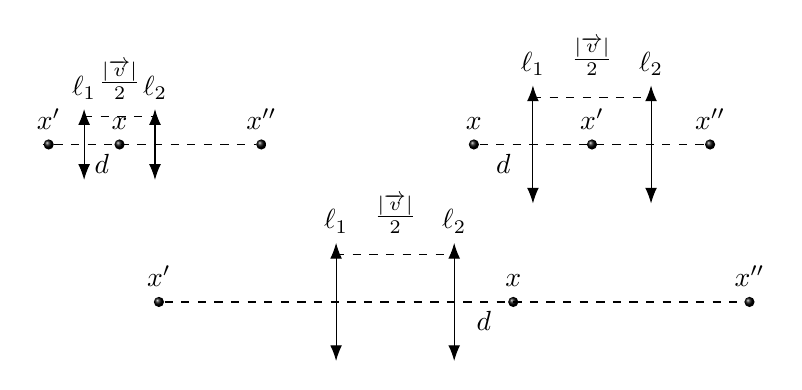
\begin{tikzpicture}
\begin{scope}[scale=0.45]
    %lines
    \draw [<->] (-1,-1) -- (-1,1);
    \draw [<->] (1,-1) -- (1,1);
    \node[above] at (-1,1) {$\ell_1$};
    \node[above] at (1,1) {$\ell_2$};
    %points
    \node[ball, label={$x$}] (x) at (0,0) {};
    \node[ball, label={$x'$}] (x') at (-2,0) {};
    \node[ball, label={$x''$}] (x'') at (4,0) {};
    \draw[dashed] (x') to (x'');
    %labels
    \node[below] at (-0.5,0) {$d$};
    \draw[dashed] (-1,0.8) to (1,0.8);
    \node[above] at (0,1) {$\frac{|\overrightarrow{v}|}{2}$};
\end{scope}
\begin{scope} [xshift=6cm,scale=0.75]
    %lines
    \draw [<->] (-1,-1) -- (-1,1);
    \draw [<->] (1,-1) -- (1,1);
    \node[above] at (-1,1) {$\ell_1$};
    \node[above] at (1,1) {$\ell_2$};
    %points
    \node[ball, label={$x$}] (x) at (-2,0) {};
    \node[ball, label={$x'$}] (x') at (0,0) {};
    \node[ball, label={$x''$}] (x'') at (2,0) {};
    \draw[dashed] (x) to (x'');
    %labels
    \node[below] at (-1.5,0) {$d$};
    \draw[dashed] (-1,0.8) to (1,0.8);
    \node[above] at (0,1) {$\frac{|\overrightarrow{v}|}{2}$};
\end{scope}
\begin{scope} [xshift=3.5cm,yshift=-2cm,scale=0.75]
    %lines
    \draw [<->] (-1,-1) -- (-1,1);
    \draw [<->] (1,-1) -- (1,1);
    \node[above] at (-1,1) {$\ell_1$};
    \node[above] at (1,1) {$\ell_2$};
    %points
    \node[ball, label={$x$}] (x) at (2,0) {};
    \node[ball, label={$x'$}] (x') at (-4,0) {};
    \node[ball, label={$x''$}] (x'') at (6,0) {};
    \draw[dashed] (x') to (x'');
    %labels
    \node[below] at (1.5,0) {$d$};
    \draw[dashed] (-1,0.8) to (1,0.8);
    \node[above] at (0,1) {$\frac{|\overrightarrow{v}|}{2}$};
\end{scope}
\end{tikzpicture}
\end{document}
    \caption{Cases (1), (2), and (3)}
\end{figure}

\end{proof}
\begin{proof}
We will consider two cases: 1) all three lines are parallel, 2) not all lines are parallel (although two of the three may be parallel to one another).
\begin{enumerate}[label=(\arabic*)]
    \item All three lines are parallel. Notice that $R_{\ell_3}\circ R_{\ell_2}\circ R_{\ell_1}=R_{\ell_3}\circ (R_{\ell_2}\circ R_{\ell_1})$, and the composition $R_{\ell_2}\circ R_{\ell_1}$ of two reflections in parallel lines is a parallel transport. By \ref{3.1} this parallel transport depends only on the direction of the lines and the distance between them, i.e. $R_{\ell_2}\circ R_{\ell_1}=R_{\ell_2'}\circ R_{\ell_1'}$. Thus, we can translate the lines $\ell_2$ and $\ell_1$ to make the second line coincide with the third, i.e. $\ell_2'=\ell_3$. Then
    \[R_{\ell_3}\circ R_{\ell_2}\circ R_{\ell_1}=R_{\ell_3}\circ R_{\ell_2'}\circ R_{\ell_1'}=R_{\ell_3}\circ R_{\ell_3}\circ R_{\ell_1'}=R_{\ell_1'}.\]
    Therefore, the result is a sliding symmetry $R_{\ell_1'}\circ T_{\overrightarrow{v}}$ where $\overrightarrow{v}=\overrightarrow{0}$.
    
    \begin{figure}[h]
        \centering
        \documentclass{standalone}
\usepackage{tikz}
%------------tikz Setup------------

\tikzstyle{ball} = [circle,shading=ball, ball color=black,
    minimum size=1mm,inner sep=1.3pt]
\tikzstyle{miniball} = [circle,shading=ball, ball color=black,
    minimum size=1mm,inner sep=0.5pt]
\tikzstyle{mminiball} = [circle,shading=ball, ball color=black,
    minimum size=0.6mm,inner sep=0.1pt]
\usetikzlibrary{arrows.meta}
\usetikzlibrary{angles, quotes}
\tikzset{>={Latex[length=2mm,width=1.5mm]}}
\tikzset{->-/.style={decoration={markings, mark=at position #1 with
  {\arrow{>}}},postaction={decorate}}}
\usetikzlibrary{decorations.pathmorphing}
\usetikzlibrary{decorations.pathreplacing}
\usetikzlibrary{arrows.meta,calc}
\usetikzlibrary{bending}
\usetikzlibrary{decorations.markings,shapes.geometric}
\tikzset{->-/.style={decoration={markings, mark=at position #1 with
  {\arrow{>}}},postaction={decorate}}}
\tikzset{-|-/.style={decoration={markings, mark=at position #1 with
  {\arrow{stealth}}},postaction={decorate}}}
\tikzset{movearrow/.style 2 args ={
        decoration={markings,
    mark= at position {#1} with {\arrow{#2}} ,
        },
        postaction={decorate}
    }
}


\begin{document}
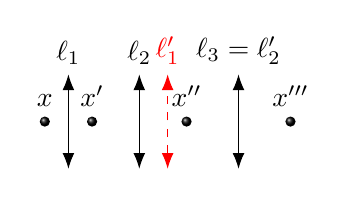
\begin{tikzpicture}
\begin{scope}[scale=0.6]
    %lines
    \draw [<->] (-1,-1) -- (-1,1);
    \draw [<->] (0.5,-1) -- (0.5,1);
    \draw [<->] (2.6,-1) -- (2.6,1);
    \draw [<->, dashed, red] (1.1,-1) -- (1.1,1);
    %labels
    \node[above] at (-1,1) {$\ell_1$};
    \node[above] at (0.5,1) {$\ell_2$};
    \node[above] at (2.6,1) {$\ell_3=\ell_2'$};
    \node[above,red] at (1.1,1) {$\ell_1'$};
    %points
    \node[ball, label={$x$}] (x) at (-1.5,0) {};
    \node[ball, label={$x'$}] (x') at (-0.5,0) {};
    \node[ball, label={$x''$}] (x'') at (1.5,0) {};
    \node[ball, label={$x'''$}] (x''') at (3.7,0) {};
\end{scope}
\end{tikzpicture}
\end{document}
        \caption{All three lines are parallel}
    \end{figure}
    
    \item Not all lines are parallel. Then the second line $\ell_2$ is not parallel to $\ell_1$ or $\ell_3$. Suppose that $\ell_1$ and $\ell_2$ are not parallel (the other case is very similar). Then the composition $R_{\ell_2}\circ R_{\ell_1}$ of reflections about intersecting lines is a rotation that depends only on the point where the lines intersect and the angle at which they intersect. So the lines $\ell_1, \ell_2$ can be rotated simultaneously about their intersection point by the same angle without changing the composition.
    \par By an appropriate rotation, make the second line $\ell_2$ perpendicular to the third line $\ell_3$, i.e. replace $\ell_1,\ell_2$ by $\ell_1',\ell_2'$ so that $R_{\ell_2}\circ R_{\ell_1}=R_{\ell_2'}\circ R_{\ell_1'}$ and $\ell_2' \perp \ell_3$.
    
    \begin{figure}[h]
        \centering
        \documentclass{standalone}
\usepackage{tikz}
%------------tikz Setup------------

\tikzstyle{ball} = [circle,shading=ball, ball color=black,
    minimum size=1mm,inner sep=1.3pt]
\tikzstyle{miniball} = [circle,shading=ball, ball color=black,
    minimum size=1mm,inner sep=0.5pt]
\tikzstyle{mminiball} = [circle,shading=ball, ball color=black,
    minimum size=0.6mm,inner sep=0.1pt]
\usetikzlibrary{arrows.meta}
\usetikzlibrary{angles, quotes}
\tikzset{>={Latex[length=2mm,width=1.5mm]}}
\tikzset{->-/.style={decoration={markings, mark=at position #1 with
  {\arrow{>}}},postaction={decorate}}}
\usetikzlibrary{decorations.pathmorphing}
\usetikzlibrary{decorations.pathreplacing}
\usetikzlibrary{arrows.meta,calc}
\usetikzlibrary{bending}
\usetikzlibrary{decorations.markings,shapes.geometric}
\tikzset{->-/.style={decoration={markings, mark=at position #1 with
  {\arrow{>}}},postaction={decorate}}}
\tikzset{-|-/.style={decoration={markings, mark=at position #1 with
  {\arrow{stealth}}},postaction={decorate}}}
\tikzset{movearrow/.style 2 args ={
        decoration={markings,
    mark= at position {#1} with {\arrow{#2}} ,
        },
        postaction={decorate}
    }
}


\begin{document}
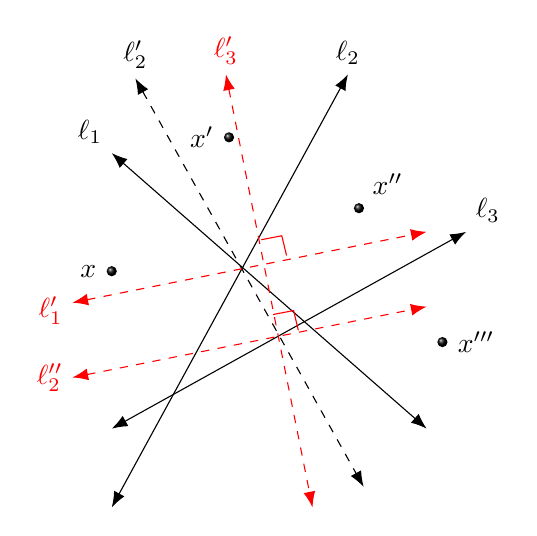
\begin{tikzpicture}
\begin{scope}[scale=1]
    %lines
    \draw [<->] (-2,-1) -- (2.5,1.5);
    \draw [<->] (-2,-2) -- (1,3.5);
    \draw [<->] (-2,2.5) -- (2,-1);
    \draw [<->,dashed] (-1.7,3.45) -- (1.2,-1.74);
    \draw [<->,dashed,red] (-2.5,0.6) -- (2,1.5);
    \draw [<->,dashed,red] (-2.5,-0.35) -- (2,0.55);
    \draw [<->, dashed,red] (-0.55,3.5) -- (0.55,-2);
    %right angles
    \draw[red] (-0.1,1.4) -- (0.16,1.45) -- (0.22,1.2);
    \draw[red] (0.05,0.45) -- (0.31,0.5) -- (0.37,0.25);
    %labels
    \node[above left] at (-2,2.5) {$\ell_1$};
    \node[above] at (1,3.5) {$\ell_2$};
    \node[above right] at (2.5,1.5) {$\ell_3$};
    \node[above] at (-1.7,3.45) {$\ell_2'$};
    \node[left,red] at (-2.5,0.5) {$\ell_1'$};
    \node[left,red] at (-2.5,-0.35) {$\ell_2''$};
    \node[above,red] at (-0.55,3.5) {$\ell_3'$};
    %points
    \node[ball, label={left:$x$}] (x) at (-2,1) {};
    \node[ball, label={left:$x'$}] (x') at (-0.51,2.7) {};
    \node[ball, label={above right:$x''$}] (x'') at (1.14,1.8) {};
    \node[ball, label={right:$x'''$}] (x''') at (2.2,0.1) {};
\end{scope}
\end{tikzpicture}
\end{document}
        \caption{Not all three lines are parallel}
    \end{figure}
    
    \par Then by rotating these two perpendicular lines $\ell_2'$ and $\ell_3$ about their intersection point, make the middle line $\ell_2''$ parallel to the line $\ell_1'$, i.e. replace $\ell_2',\ell_3$ by $\ell_2'',\ell_3'$ so that 
    \[R_{\ell_3}\circ R_{\ell_2}\circ R_{\ell_1}=R_{\ell_3}\circ R_{\ell_2'}\circ R_{\ell_1'}=R_{\ell_3'}\circ R_{\ell_2''}\circ R_{\ell_1'}.\]
    \par Now, the configuration has $\ell_1', \ell_2''$ parallel, $\ell_3'$ is perpendicular to them both. By lemma \ref{3.1}, $R_{\ell_2''}\circ R_{\ell_1'}$ is a translation by a vector perpendicular to them both and parallel to $\ell_3'$, so $R_{\ell_3'}\circ R_{\ell_2''}\circ R_{\ell_1'}=R_{\ell_3}\circ R_{\ell_2}\circ R_{\ell_1}$ is a sliding symmetry.
\end{enumerate}
\end{proof}


\section{Problem 4.}
The points $A_1,A_2,\dots,A_n$ form a regular polygon inscribed in a circle with the center $O$. A point $X$ lies on the same circle. Prove that the images of the point $X$ under the symmetries with axes $OA_1,OA_2,\dots,OA_n$ form a regular polygon.
\begin{proof}
Without loss of generality (since $A_1,A_2,\dots,A_n$ form a regular polygon), let $A_1$ be the closest point to $X$. Then the angle $\theta=\angle XOA_1$ is the smallest angle between $X$ and any other point.

\begin{figure}[h]
    \centering
    \documentclass{standalone}
\usepackage{tikz}
%------------tikz Setup------------

\tikzstyle{ball} = [circle,shading=ball, ball color=black,
    minimum size=1mm,inner sep=1.3pt]
\tikzstyle{miniball} = [circle,shading=ball, ball color=black,
    minimum size=1mm,inner sep=0.5pt]
\tikzstyle{mminiball} = [circle,shading=ball, ball color=black,
    minimum size=0.6mm,inner sep=0.1pt]
\usetikzlibrary{arrows.meta}
\usetikzlibrary{angles, quotes}
\tikzset{>={Latex[length=2mm,width=1.5mm]}}
\tikzset{->-/.style={decoration={markings, mark=at position #1 with
  {\arrow{>}}},postaction={decorate}}}
\usetikzlibrary{decorations.pathmorphing}
\usetikzlibrary{decorations.pathreplacing}
\usetikzlibrary{arrows.meta,calc}
\usetikzlibrary{bending}
\usetikzlibrary{decorations.markings,shapes.geometric}
\tikzset{->-/.style={decoration={markings, mark=at position #1 with
  {\arrow{>}}},postaction={decorate}}}
\tikzset{-|-/.style={decoration={markings, mark=at position #1 with
  {\arrow{stealth}}},postaction={decorate}}}
\tikzset{movearrow/.style 2 args ={
        decoration={markings,
    mark= at position {#1} with {\arrow{#2}} ,
        },
        postaction={decorate}
    }
}


\begin{document}
 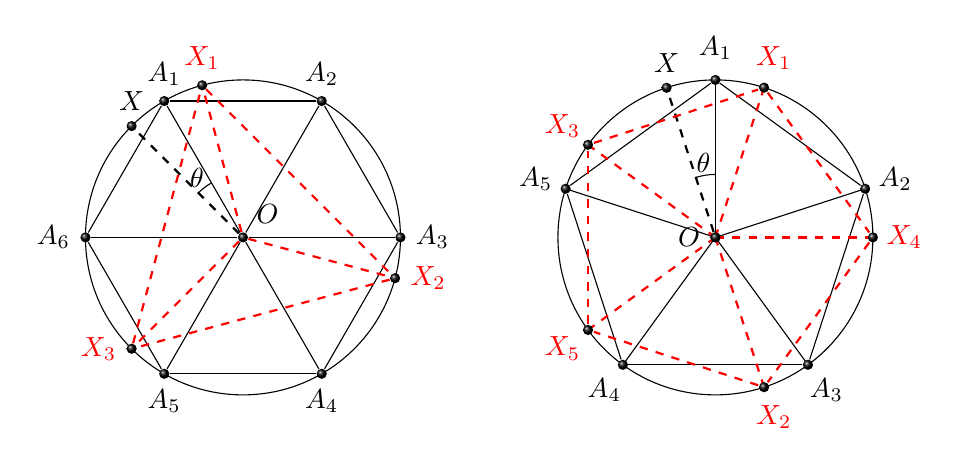
\begin{tikzpicture}
\begin{scope}
    \draw (0,0) circle [radius=2]; %circle
    \node[ball,label={above right:$O$}] (o) at (0,0) {};  %center
    \node[ball,label={above:$X$}] (x) at (-1.414, 1.414) {};    %X
    %original hexagon
    \node[ball,label={above:$A_1$}] (1) at (-1, 1.732) {};
    \node[ball,label={above:$A_2$}] (2) at (1, 1.732) {};
    \node[ball,label={right:$A_3$}] (3) at (2, 0) {};
    \node[ball,label={below:$A_4$}] (4) at (1, -1.732) {};
    \node[ball,label={below:$A_5$}] (5) at (-1, -1.732) {};
    \node[ball,label={left:$A_6$}] (6) at (-2, 0) {};
    \draw (1) to (2);
    \draw (2) to (3);
    \draw (3) to (4);
    \draw (4) to (5);
    \draw (5) to (6);
    \draw (6) to (1);
    \draw (o) to (1);
    \draw (o) to (2);
    \draw (o) to (3);
    \draw (o) to (4);
    \draw (o) to (5);
    \draw (o) to (6);
    %rotated triangle
    \node[ball,label={above, red:$X_1$}] (x1) at (-0.518, 1.932) {};
    \node[ball,label={right, red:$X_2$}] (x2) at (1.932, -0.518) {};
    \node[ball,label={left, red:$X_3$}] (x3) at (-1.414, -1.414) {};
    \draw[dashed, thick] (o) to (x);
    \draw[dashed, red, thick] (o) to (x1);
    \draw[dashed, red, thick] (o) to (x2);
    \draw[dashed, red, thick] (o) to (x3);
    \draw[dashed, red, thick] (x1) to (x2);
    \draw[dashed, red, thick] (x2) to (x3);
    \draw[dashed, red, thick] (x3) to (x1);
    % angle
    \pic [draw,
          angle radius=8mm, angle eccentricity=1.2,
          "$\theta$"] {angle = 1--o--x};
\end{scope}
\begin{scope}[xshift=6cm,scale=2]
    \draw (0,0) circle [radius=1];  %circle
    \node[ball,label={left:$O$}] (o) at (0,0) {};   %center
    \node[ball,label={above:$X$}] (x) at (-0.31,0.95) {};   %X
    \draw[dashed, thick] (o) to (x);
    \def\deg{72}    %interior angle
    %original pentagon
    \foreach [evaluate={
        \t=int(162-\x*\deg);
        }]\x in {1,2,...,5}
    {\draw (0:0)--(\t:1) node[ball] (\x) at (\t:1) {};
    \node[anchor=center] at (\t:1.2) {$A_{\x}$};}
    \foreach \from/\to in {1/2, 2/3, 3/4, 4/5, 5/1}
    {\draw (\from) -- (\to);}
    % angle
    \pic [draw,
          angle radius=8mm, angle eccentricity=1.2,
          "$\theta$"] {angle = 1--o--x};
    %rotated pentagon
    \foreach [evaluate={
        \t=int(144-\x*\deg);
        \p=int(72-2*(\x-1)*\deg);
        }]\x in {1,2,...,5}
    {\draw[dashed, red, thick] (0:0)--(\t:1) node[ball] (\x) at (\t:1) {};
    \node[anchor=center, red] at (\p:1.2) {$X_{\x}$};}
    \foreach \from/\to in {1/2, 2/3, 3/4, 4/5, 5/1}
    {\draw[dashed, red, thick] (\from) -- (\to);}
    \node[ball] at (0,0) {};
\end{scope}
\end{tikzpicture}
\end{document}
    \caption{Example of a hexagon and pentagon.}
\end{figure}

\par For the rest of the proof, we will consider all angles with respect to segment $OA_1$. Reflecting $X$ across axis $OA_1$ to $X_1$ yields $\angle X_1OA_1=\theta$. The interior angle of a regular polygon of $n$ sides is $\frac{2\pi}{n}$, so reflecting $X$ across axis $OA_2$ to $X_2$ yields $\angle X_2OA_1=\theta+2\frac{2\pi}{n}$. Performing reflections along each axis $OA_1,OA_2,\dots,OA_n$ yields the following angles: 
\[\theta, \theta+2\frac{2\pi}{n}, \theta+4\frac{2\pi}{n}, \dots, \theta+2(n-1)\frac{2\pi}{n}.\]
\par For even $n$, subtracting $\theta$ and taking modulo $2\pi$ for all angles gives \[0, \frac{4\pi}{n}, \frac{8\pi}{n}, \dots, 2\pi -\frac{4\pi}{n}.\]
\par For odd $n$, subtracting $\theta$ and taking modulo $2\pi$ for all angles gives \[0, \frac{2\pi}{n}, \frac{4\pi}{n}, \dots, 2\pi -\frac{2\pi}{n}.\]
\par Thus for even $n$, the angles have difference $\frac{4\pi}{n}$, so the images $X_i$ form a regular polygon with $\frac{n}{2}$ sides. For odd $n$, the angles have difference $\frac{2\pi}{n}$, so the images $X_i$ form a regular polygon with $n$ sides.
\end{proof}


\section{Problem 5.}
Remove a corner from a $101\times 101$ chessboard. Prove that the rest of the board cannot be covered by triominoes. A triomino is like a domino except it consists of three squares in a row; each cell can cover one cell on the chessboard. Each triomino can either "stand" or "lie."
\begin{proof}
We can recolor the $101\times 101=10201$ tiles of the chessboard with three colors, red, yellow, and blue. We can recolor by alternating the colors of the diagonals, blue, red, yellow, starting with red on the longest diagonal of $101$ squares. Then there are $101+2(98+95+\dots+2)=101+2 \left (\frac{100\times 33}{2}\right )=3401$ red tiles. By symmetry, there are $\frac{10201-3401}{2}=3400$ of each blue and yellow tiles. Without loss of generality, let us remove a blue corner. Then there are $3401$ red, $3400$ yellow, and $3399$ blue tiles.

\begin{figure}[h]
    \centering
    \documentclass{standalone}
\usepackage{tikz}
%------------tikz Setup------------

\tikzstyle{ball} = [circle,shading=ball, ball color=black,
    minimum size=1mm,inner sep=1.3pt]
\tikzstyle{miniball} = [circle,shading=ball, ball color=black,
    minimum size=1mm,inner sep=0.5pt]
\tikzstyle{mminiball} = [circle,shading=ball, ball color=black,
    minimum size=0.6mm,inner sep=0.1pt]
\usetikzlibrary{arrows.meta}
\usetikzlibrary{angles, quotes}
\tikzset{>={Latex[length=2mm,width=1.5mm]}}
\tikzset{->-/.style={decoration={markings, mark=at position #1 with
  {\arrow{>}}},postaction={decorate}}}
\usetikzlibrary{decorations.pathmorphing}
\usetikzlibrary{decorations.pathreplacing}
\usetikzlibrary{arrows.meta,calc}
\usetikzlibrary{bending}
\usetikzlibrary{decorations.markings,shapes.geometric}
\tikzset{->-/.style={decoration={markings, mark=at position #1 with
  {\arrow{>}}},postaction={decorate}}}
\tikzset{-|-/.style={decoration={markings, mark=at position #1 with
  {\arrow{stealth}}},postaction={decorate}}}
\tikzset{movearrow/.style 2 args ={
        decoration={markings,
    mark= at position {#1} with {\arrow{#2}} ,
        },
        postaction={decorate}
    }
}


\begin{document}
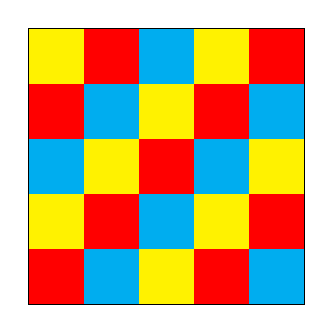
\begin{tikzpicture}[scale=0.7]
    \draw[thick] (0,0) rectangle (5,5);
    \fill[red] (0,0) rectangle (1,1);
    \fill[red] (1,1) rectangle (2,2);
    \fill[red] (2,2) rectangle (3,3);
    \fill[red] (3,3) rectangle (4,4);
    \fill[red] (4,4) rectangle (5,5);
    \fill[red] (3,0) rectangle (4,1);
    \fill[red] (4,1) rectangle (5,2);
    \fill[red] (0,3) rectangle (1,4);
    \fill[red] (1,4) rectangle (2,5);
    \fill[cyan] (1,0) rectangle (2,1);
    \fill[cyan] (2,1) rectangle (3,2);
    \fill[cyan] (3,2) rectangle (4,3);
    \fill[cyan] (4,3) rectangle (5,4);
    \fill[cyan] (0,2) rectangle (1,3);
    \fill[cyan] (1,3) rectangle (2,4);
    \fill[cyan] (2,4) rectangle (3,5);
    \fill[cyan] (4,0) rectangle (5,1);
    \fill[yellow] (0,1) rectangle (1,2);
    \fill[yellow] (1,2) rectangle (2,3);
    \fill[yellow] (2,3) rectangle (3,4);
    \fill[yellow] (3,4) rectangle (4,5);
    \fill[yellow] (2,0) rectangle (3,1);
    \fill[yellow] (3,1) rectangle (4,2);
    \fill[yellow] (4,2) rectangle (5,3);
    \fill[yellow] (0,4) rectangle (1,5);
\end{tikzpicture}
\end{document}
    \caption{Bottom left corner section of the tri-colored chessboard}
\end{figure}

\par We notice that in this coloring, whether a triomino is in the "stand" or "lie" position, it must cover one red, one yellow, and one blue tile. After using up $3399$ triominoes, we will have covered $3399$ of each color, leaving two red and one yellow tile, which is impossible to cover with the last needed triomino.
\end{proof}


\section{Problem 6.}
Consider a finite collection of segments on a line so that every two of them intersect. Prove that all segments have a common point.
\begin{proof}
Let for $1\leq i,j\leq k$, let $S_i$ and $S_j$ be segments and $a_{ij}=a_{ji}$ be any point on $S_i \cap S_j$. Then let 
\begin{align*}
    b_1&=\max_{1 \leq i \leq k}\min_{1 \leq j \leq k}a_{ij}.\\ 
    b_2&=\min_{1 \leq i \leq k}\max_{1 \leq j \leq k}a_{ij}.
\end{align*}
\par That is, between each intersections $S_i \cap S_j$, take the smallest and largest $a_{ij}$. Then $b_1$ is the largest of the set of smallest intersection points, and $b_2$ is the smallest of the set of largest intersection points.
\par We can show that $b_1 \leq b_2$. Take any indices $i_1$ and $i_2$. Then $b_1=\min_{1 \leq j \leq k}a_{i_1j}$ and $b_2=\max_{1 \leq j \leq k}a_{i_2j}$. Hence, $b_1\leq a_{i_1i_2} = a_{i_2i_1}\leq b_2$.
\par Finally, we can show any point $p\in [b_1,b_2]$ is a common point of every segment. For any segment $S_i$, we have $p\leq b_2=\max_{1 \leq j \leq k}a_{ij} \in S_i$, so $p$ is less than or equal to at least one point in every $S_i$. Furthermore, we have $p\geq b_1=\min_{1 \leq j \leq k}a_{ij} \in S_i$, so $p$ is greater than or equal to at least one point in every $S_i$. Thus, $p$ is in every segment, so all segments have at least one common point $p$.
\end{proof}


\section{Problem 7.}
Let $S$ be a set of $n+1$ integers from $1$ to $2n$. Prove that at least two elements in S are coprime.
\begin{proof}
We can divide the integers into pairs: $\{1,2\},\{3,4\},\dots,\{2n-1,2n\}$. By the pigeonhole principle, when we select $n+1$ integers, at least two must be in the same pair. Thus, we must have at least one pair of consecutive integers.
\par We can show that two consecutive integers $n$ and $n+1$ are necessarily coprime. Suppose $gcd(n,n+1)=p$. Then $p|n$ and $p|n+1$, so $p|n+1-n$ or $p|1$. Then $p=1$, and $gcd(n,n+1)=1$, so $n$ and $n+1$ are coprime. 
\par Hence, at least two elements in $S$ are coprime. 
\end{proof}


\end{document}
